%%%%%%%%%%%%%%%%%%%%%%%%%%%%%%%%%%%%%%%%%%%%%%%%%%%%%%%%%%%%%%%%%%%%%%%%%%%%%%%%%%%%%%%%%
% Appendix A: XDLRC Syntax
%	This section provides a detailed description of XDLRC files, and their syntax.
%	Most users of RS2 don't need to know the syntax of XDLRC files, but
% 	this information may be useful to new lab members working on the project.
%%%%%%%%%%%%%%%%%%%%%%%%%%%%%%%%%%%%%%%%%%%%%%%%%%%%%%%%%%%%%%%%%%%%%%%%%%%%%%%%%%%%%%%%%
\newpage
\appendix
\section{XDLRC Files and Syntax} \label{sec:appendixXDLRC}
In general, users of RS2 do not need to understand the syntax of XDLRC
files to create CAD tools in RS2. The syntax is introduced here for those
who are interested, and for those who want to modify the XDLRC parser
in some way. If these don't apply to you, then go ahead and skip this section.
XDLRC files are textual descriptions of Xilinx FPGA devices and can be very
verbose (which is why they get so large). This section highlights the main parts
of an XDLRC file with accompanying images. As you will see, much of the
terminology is the same as \autoref{fpgaArch}.

\bigbreak \noindent
\begin{large}
\pgm{Tiles}
\end{large}

\begin{figure}[H]
	\centering
	
\includegraphics[width=1\columnwidth]{xdlrcTile}
	\caption{Tile syntax in XDLRC files}
	\label{fig:xdlrcTile}
\end{figure}

\noindent
A tile in an XDLRC file corresponds to the same thing as the \cls{Tile}
described in \autoref{fpgaArch}. Each tile is declared with a ``(tile''
directive as shown above followed by the unique row and column index of where
the tile fits into the grid of tiles found on the FPGA. The tile declaration
also contains a name followed by a type with the final number being the number
of primitive sites found within the tile. The tile ends with a ``tile\_summary''
statement repeating the name and type with some other numbered statistics.
Tiles can contain three different sub components, primitive sites, wires, and
PIPs.

\bigbreak \noindent
\begin{large}
\pgm{Primitive Sites}
\end{large}

\begin{figure}[H]
	\centering
	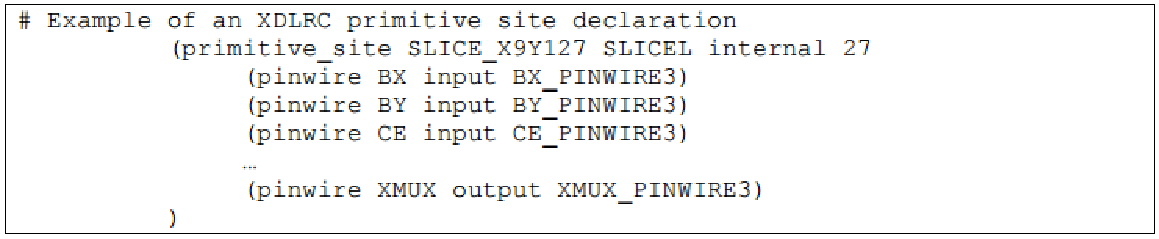
\includegraphics[width=1\columnwidth]{xdlrcSite}
	\caption{Primitive site syntax in XDLRC files}
	\label{fig:xdlrcSite}
\end{figure}

\noindent
Primitive site declarations in XDLRC files contain a list of pinwires which
describe the name and direction of pins on the primitive site. The first
pinwire declared in the example above is the BX input pin which is the internal
name to the SLICEL primitive site. Pinwires have an external name as well to
differentiate the multiple primitive sites that may be present in the same
tile. In this case, BX of SLICE\_X9Y127 has the external name BX\_PINWIRE3. In
RS2, only the first pin name (i.e. BX above) is used.

\bigbreak \noindent
\begin{large}
\pgm{Wire}
\end{large}

\begin{figure}[H]
	\centering
	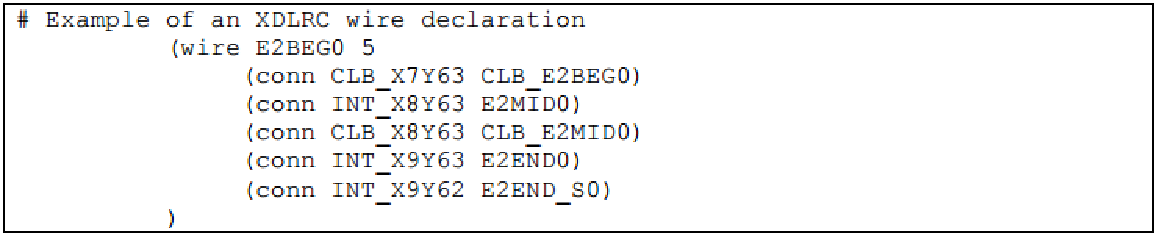
\includegraphics[width=1\columnwidth]{xdlrcWire}
	\caption{Wire syntax in XDLRC files}
	\label{fig:xdlrcWire}
\end{figure}

\noindent
A wire as declared in XDLRC is a routing resource that exists in the tile that
may have zero or more connections leaving the tile. In the example above, the
wire ``E2BEG0'' connects to 5 neighboring tiles. These connections (denoted
by ``conn'') are described using the unique tile name and wire name of that tile
to denote connectivity. The connections are not programmable, but hard wired
into the FPGA. Wire portions of the XDLRC file are included in the definition of
every tile (even if the same tile type has already been printed), which has a
big impact on the final size of XDLRC files. How RS2 handles wire
duplication is described in \autoref{wireEnum}. The \cls{WireConnection}
objects that are created from this part of the XDLRC are described in
\autoref{wireConnSection}.

\bigbreak \noindent
\begin{large}
\pgm{PIP}
\end{large}

\begin{figure}[H]
	\centering
	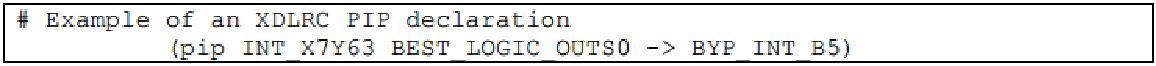
\includegraphics[width=1\columnwidth]{xdlrcPip}
	\caption{PIP syntax in XDLRC files}
	\label{fig:xdlrcPip}
\end{figure}

\noindent
A PIP (programmable interconnect point) is a possible connection that can be
made between two wires. In the example above, the PIP is declared in the tile
and repeats the tile name for reference. It specifies two wires by name that
both exist in that same tile (``BEST\_LOGIC\_OUTS0'' and ``BYP\_INT\_B5'') and
declares that the wire ``BEST\_LOGIC\_OUTS0'' can drive the wire
``BYP\-\_INT\_B5''. A collection of these PIPs in a net define how a net is
routed and is consistent with saying that those PIPs are �turned on.�
\autoref{wireConnSection} describes in detail how PIPs are represented in
RS2.

\bigbreak \noindent
\begin{large}
\pgm{Primitive Definitions}
\end{large}

\bigbreak \noindent
The Primitive Definition portion of an XDLRC file textually describes the
components found within a \cls{Primitive} \cls{Site} (a SLICEL for example)
and how they are connected. This includes: 

\begin{itemize}
  \item BELs
  \item Site Pins 
  \item Site Pips (Routing Muxes) 
  \item Configuration options (both site and BEL)
  \item Site Routethroughs (configurable connections from a site input pin to
  a site output pin)
  \item Site Wire Connections
\end{itemize}

\noindent An example of a complete primitive definition file of type BUFHCE can
be seen in \autoref{fig:xdlrcDef}. The sub-site data structures in RS2
(\cls{Bels}, \cls{SiteWire}s, etc.) are built by parsing this section of the
XDLRC file. For a more detailed description of primitive definitions, view the
VSRT User Guide in the RS2 repository.

\begin{figure}[H]
	\centering
	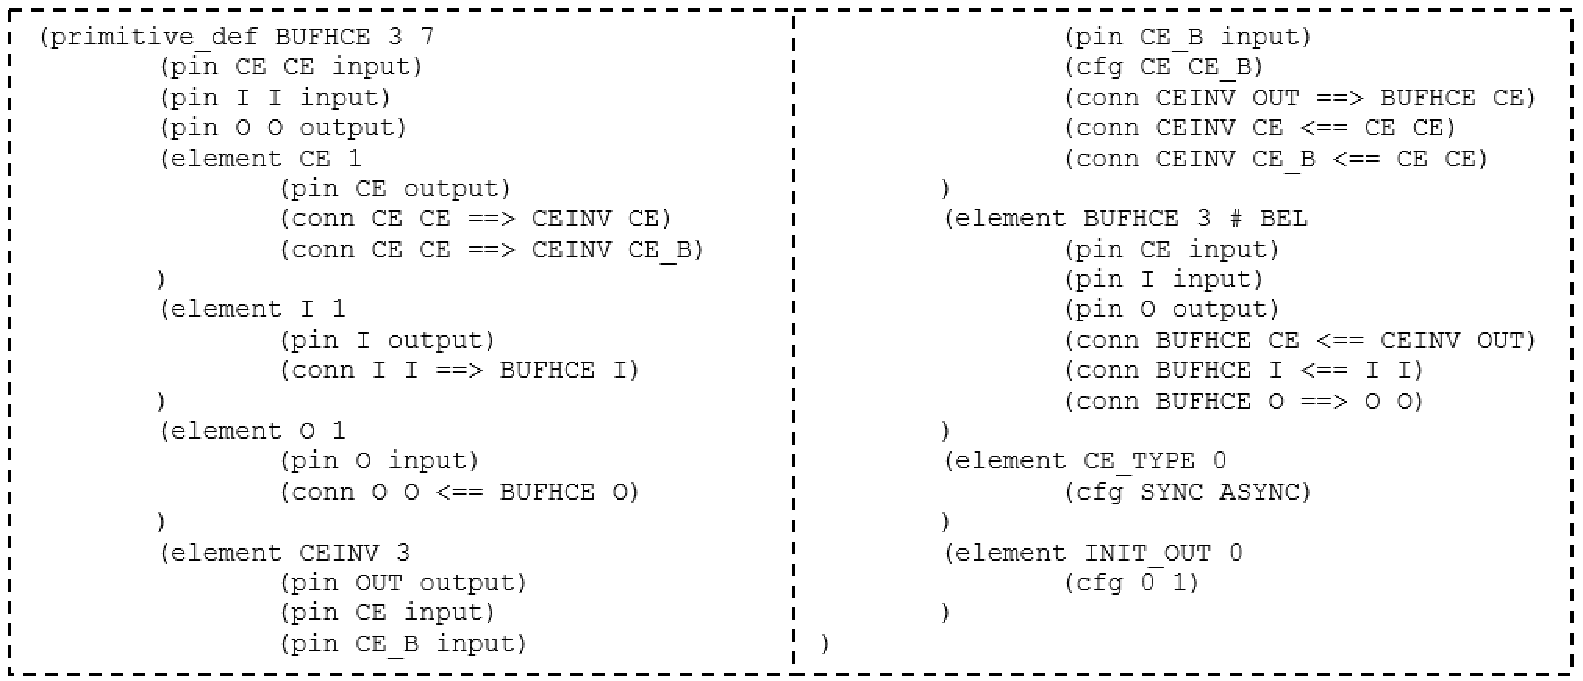
\includegraphics[width=1\columnwidth]{xdlrcDef}
	\caption{Primitive Def sections of XDLRC files}
	\label{fig:xdlrcDef}
\end{figure}
